\documentclass[12pt]{article}


\usepackage[dvips,letterpaper,margin=0.75in,bottom=0.5in]{geometry}
\usepackage{cite}
\usepackage{slashed}
\usepackage{graphicx}
\usepackage{amsmath}

\begin{document}

\section{Introduction}

In this two-week long lab, which will require a long lab write-up, you
will build the data acquisition (DAQ) unit for a Geiger counter.  You
will compare the data you collect using your custom DAQ to compare
with the theoretical expectations for Poisson and Gaussian distributed
random variables.

\begin{figure}[htbp]
\begin{center}
{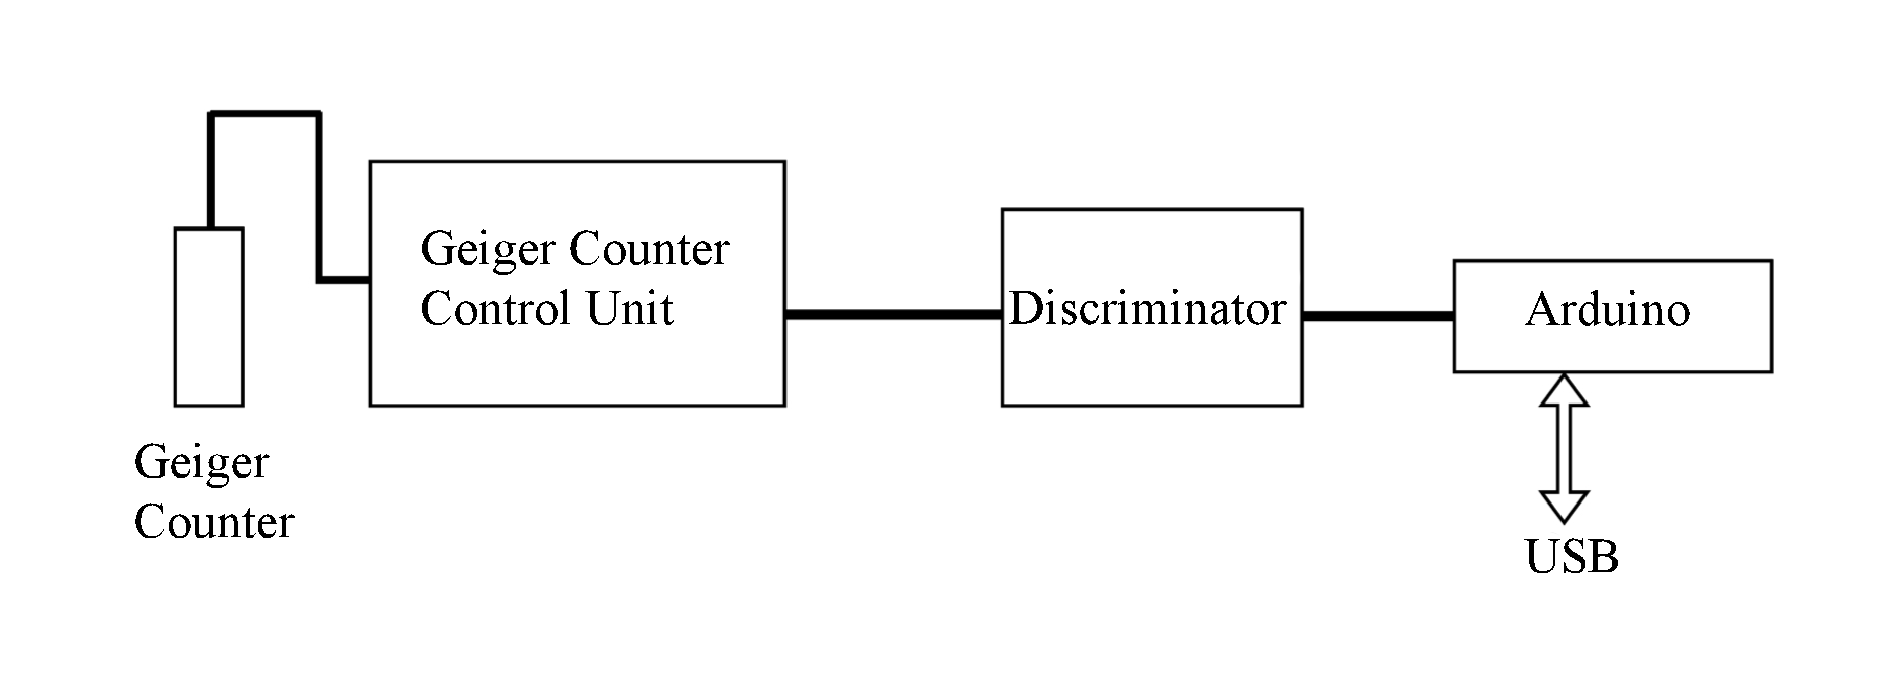
\includegraphics[width=0.75\textwidth]{figs/plan.pdf}}
\end{center}
\caption{\label{fig:plan} An overview of the lab setup.  The Geiger
  counter and control unit are provided.  You will build the
  discriminator stage and program an Arduino to complete the DAQ.}
\end{figure}

\begin{figure}[htbp]
\begin{center}
{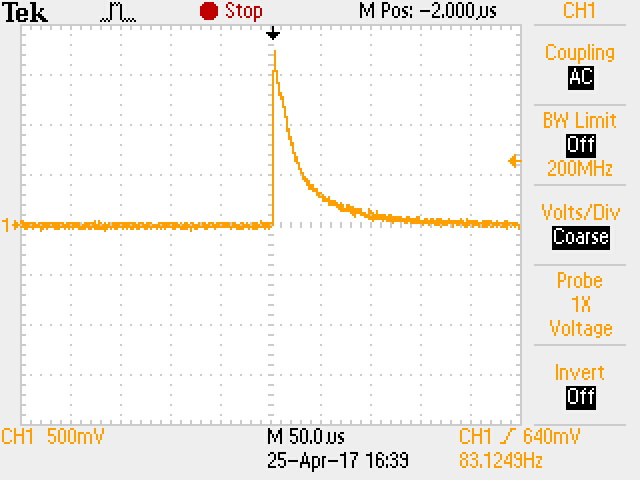
\includegraphics[width=0.55\textwidth]{figs/geiger_pulse.jpg}}
\end{center}
\caption{\label{fig:geigerpulse} Typical pulse from the Geiger counter}
\end{figure}

An overview of the lab setup is shown in Fig.~\ref{fig:plan}.  Once
properly setup, the Geiger counter will produce a pulse like the one
shown in Fig.~\ref{fig:geigerpulse} each time ionizing radiation
passes through the chamber.  The scope trace is AC-coupled, and
therefore does not show the 5 volt offset (called a pedestal) that is
present at the output.  The first stage of the discriminator removes
this pedestal with a high-pass filter.  The subsequent stages convert
these pulses above threshold into 5 volt digitized TTL pulses.  Once
connected to the Arduino, the DAQ unit receives a single TTL digital
pulse on an input pin for each incident ionizing particle.  The DAQ
simply counts these pulses during a fixed time interval and reports
the results over the serial connection.  You'll build the
discriminator, the DAQ, collect the data, analyze it using scientific
python, and report everything in a long writeup.

\section{Precautions}

\noindent
{\em Precautions with the Geiger counter:}
\begin{itemize}
\item Leave the cable from the Geiger counter controller to the Geiger counter in place {\em at all times}.  This carries voltages of approximately 1000 volts.  If you leave the cable in place, nothing can be inadvertently plugged in (including fingers!)
\item Leave the Geiger tube in its holder.  It has a thin front window which is easily broken.
\end{itemize}

\noindent
{\em Precautions with the radioactive source:}
\begin{itemize}
\item Don't touch the source.
\item Leave the source in the tray at all times.  The TA will provide the sources and handle moving them from place to place.
\item Radiation falls off as $1/r^2$.  So minimize your time near sources and maximize your distance from them.
\item Further information on radiation safety can be found in Melissinos and Napolitano.
\end{itemize}

\section{AC-coupled Schmitt trigger discriminator}

The first stage of the DAQ will be an analog-to-digital converter stage that you will build yourself based on a Schmitt trigger.  Your discriminator circuit is AC coupled, to remove the 5 volt pedestal included with the signal.  This AC coupling allows us to test the circuit efficiently using a square wave input.  The high-pass-filter converts the square wave input into current pulses much like those from the Geiger counter, but at a constant, known rate, as shown in Fig.~ref{fig:fakepulse}.

\begin{figure}[htbp]
\begin{center}
{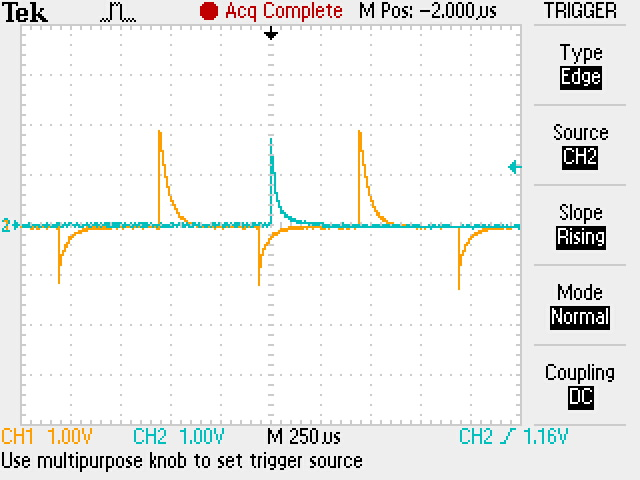
\includegraphics[width=0.55\textwidth]{figs/fake_pulse.jpg}}
\end{center}
\caption{\label{fig:fakepulse} Typical pulse (CH1) resulting from the square wave input compared to an actual pulse (CH2) from Geiger counter.
These are measured at the non-inverting input (pin 3 of the LM311 in the discriminator circuit below.)  The inverted pulses, which result from the falling edge of square wave function, are ignored by the circuit.}
\end{figure}

\begin{figure}[thbp]
\begin{center}
{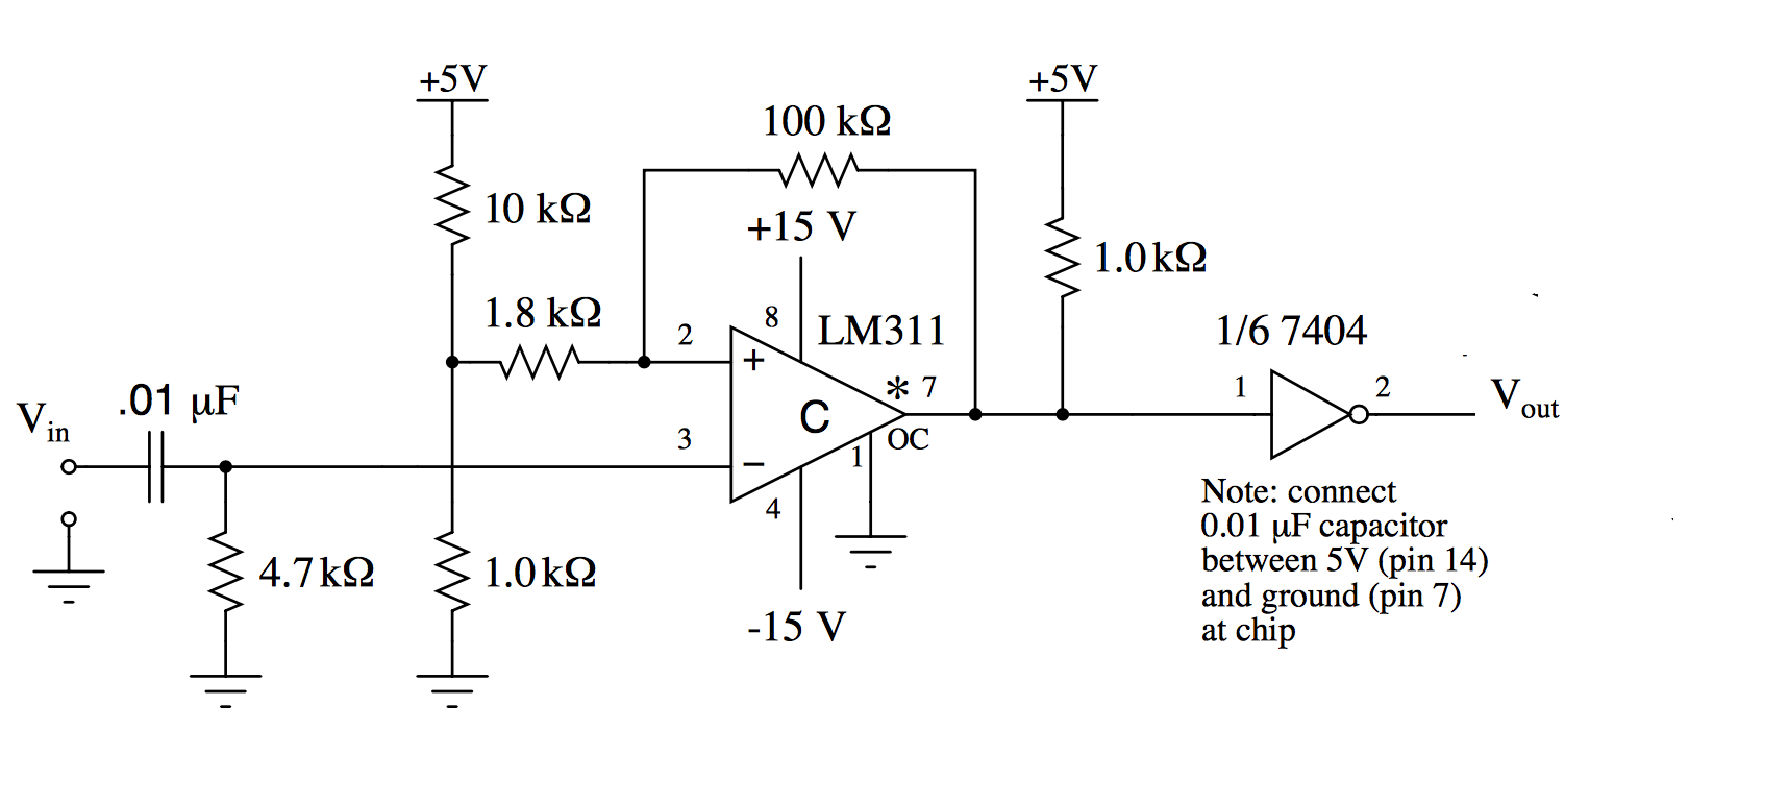
\includegraphics[width=0.75\textwidth]{figs/discrim.pdf}}
\end{center}
\caption{\label{fig:filter} Circuit diagram.}
\end{figure}

\begin{figure}[thbp]
\begin{center}
{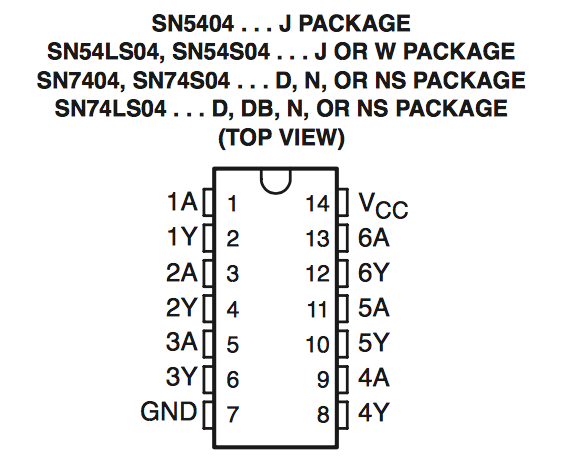
\includegraphics[width=0.35\textwidth]{figs/7404_pinout.png}}
{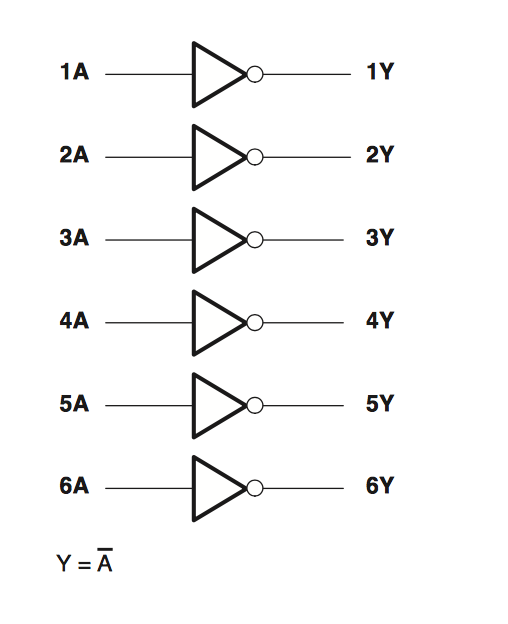
\includegraphics[width=0.25\textwidth]{figs/7404_scheme.png}}
\caption{\label{fig:7404} The 74XX04 in 14-pin DIP}
\end{center}
\end{figure}

\begin{figure}[thbp]
\begin{center}
{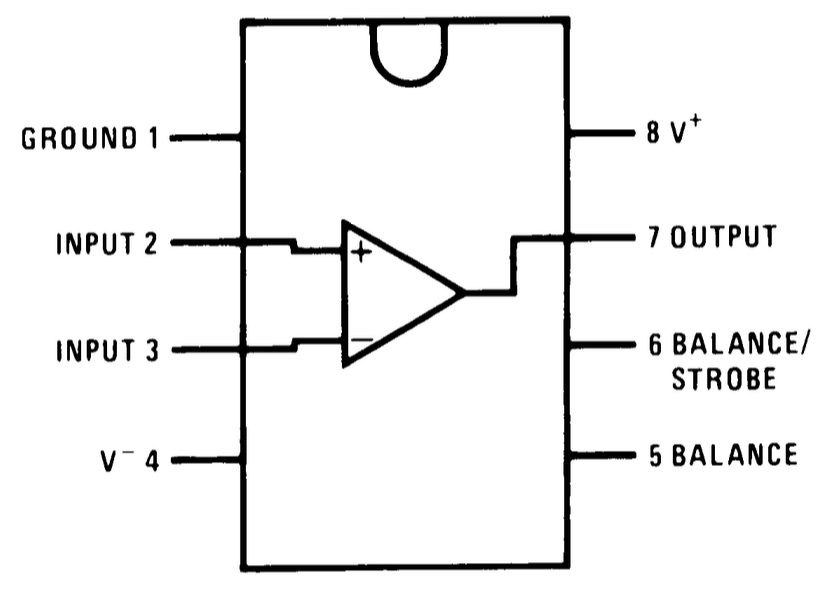
\includegraphics[width=0.40\textwidth]{figs/LM311.png}}
\caption{\label{fig:lm311} The LM311 in 8-pin PDIP.}
\end{center}
\end{figure}

\begin{figure}[htbp]
\begin{center}
{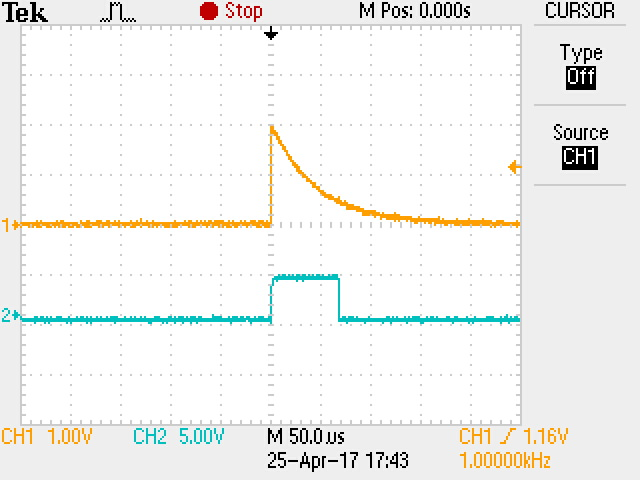
\includegraphics[width=0.55\textwidth]{figs/discrim_out.jpg}}
\end{center}
\caption{\label{fig:typout} Typical output (CH2) of the discriminator circuit (measured at $V_{\rm out}$) compared to the input (measured at the non-inverting input, pin 3 of the LM311.) }
\end{figure}

Build the circuit shown in Fig.~\ref{fig:filter} using the components in Figs.~\ref{fig:7404} and \ref{fig:lm311}.  For debugging, drive the circuit at $V_{\rm in}$ with a 1~kHz square-wave at 2 volts peak-to-peak.  Typical output from the circuit is shown in Fig.~\ref{fig:typout}.  Note the different scale:  the output is 5 volt TTL digital logic, easily handled by a microprocessor.

\section{Arduino Based DAQ}

The output of your discriminator circuit is easily handled by an Arduino microprocessor.  The signal is a digital 5 volt TTL pulse with a width of order several tens of microseconds, which can be fed directly to a digital input pin on the Arduino.  The Arduino should also be grounded to the same ground used in your discriminator circuit.  Your Arduino, if programmed correctly, can make one digital read approximately every 5 microseconds, which is plenty fast enough to handle these TTL pulses.

You should therefore design a DAQ for your Arduino which:
\begin{itemize}
\item Measures the current time in microseconds.
\item Makes a programmable number of iterations ($N_I$) reading the digital input each iteration.
\item Increments a counter ($N_C$) each time a new pulse is detected (a digital value ``1" after a ``0")
\item Measures the stop time.
\item Calculates the duration ($\tau$) of the run, from stop time minus start time.
\item On the serial bus, reports $\tau$, $N_I$, and $N_C$.
\item Repeats again from the start 100 times.
\end{itemize}
When designing your DAQ, consider the following:
\begin{itemize}
\item You might measure a ``1" corresponding to single pulse multiple times.  So the sequence 0001111110000 should increment your counter only once, not six times.
\item We are pushing the limits of the Arduino timing, so you'll want to place the loop over $N_I$ iterations directly in a for loop, which does the data collection, counting, and nothing else.  Keep it simple!  You should check that you manage to keep the sample rate $\tau / N_I$ at nearly 5 microseconds.
\item For actually collecting the data, you can simply cut and paste the serial monitor output into a text file.  It will be easiest to process the data later using scientific python if the output is simply one line per run, with the variables reported separated only by spaces.   Of course you can add whatever output you want at the beginning and end.
\item Verify that by adjusting the number of samples collected, you can control the interval $\tau$ to 100~ms and 1000~ms.
\item Verify that your Arduino consistently measures the rate that you expect, based on the square wave input that you are feeding it, and that it does not depend on the value of $\tau$.
\end{itemize}
Once you have verified that both your discriminator circuit and Arduino-based DAQ are working as expected, you are ready to start taking data.

\section{The Geiger Counter}

On the Geiger Controller, start with the HV set to zero at both the analog knob and the HV on-off switch.   Turn on the device and set the mode to``Test".  In this mode, the counter will be incremented at a fixed rate of 60 Hz.   While in this mode, play around with the ``Count", ``Reset", and ``Lab-Chron" analog timer reset dial until you understand how all of these features work.

Next check that you have a source in the second highest draw of the Geiger Counter holder, asking the TA for help if this is not the case.  Switch the mode back to ``Use", which will now use the Geiger counter as input to the count.  With the HV still off, place the controller in ``Count" mode, and verify that the rate, with no HV, is zero.  Now, with the controller still in ``Count" mode, turn on the HV and turn the dial until you first see the counter incrementing.  Turn up the voltage to the next interval of 50 volts (e.g. if it first starts incrementing at 730 volts, set the dial to 750 volts).

Tabulate the number of counts in a 10 seconds interval, twice for each voltage level, in 50 volt steps from your starting voltage up to 1000 volts.  Do not exceed 1000 volts.  From the data, select the start of the plateau region, where increasing the voltage by 50 volts raises the rate by less than $10\%$.

With another measurement, confirm that the rate at this plateau is of order 100 Hz (this will vary from source to source).

Look at the ``SCOPE" output of the Geiger counter controller on your oscilloscope, with AC coupling, and verify that you see output pulses similar to those in Fig.~\ref{fig:geigerpulse}.

\section{Connect the DAQ}

Connect the "SCOPE" output of the Geiger counter controller to the input of your discriminator circuit.  It is useful to use a BNC Tee connection at the scope so that you can continue to trigger and monitor Geiger counter pulses and drive your discriminator with the same input.  Now check the output of your discriminator and verify that you have the expected TTL output pulse, as in Fig.~\ref{fig:geigerdigitized}.  If the width of the TTL output pulse is less than 10 microseconds, your Arduino may have trouble keeping up.   If this is the case, seek help from the TA.  Together, you can try increasing the HV (but do not exceed 1000 V) and (if that fails) you could try adjusting the capacitance of the high-pass filter stage.

\begin{figure}[htbp]
\begin{center}
{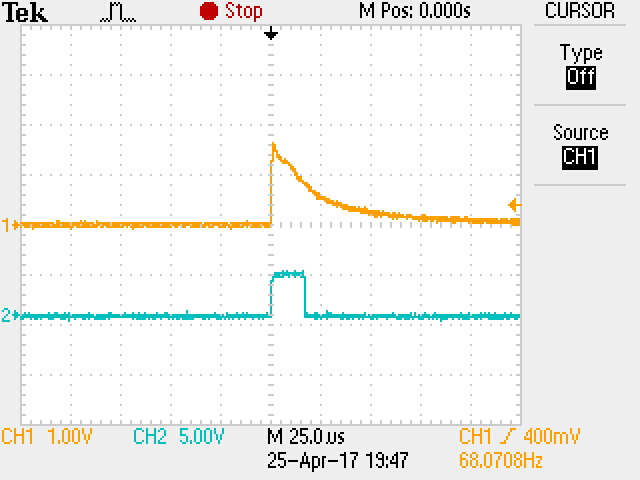
\includegraphics[width=0.55\textwidth]{figs/geiger_digitized.jpg}}
\end{center}
\caption{\label{fig:geigerdigitized} Response of the discriminator stage (CH2) to a pulse from the Geiger counter (CH1).}
\end{figure}


With the shape of the digital input pulse verified, plug this in as input to your Arduino DAQ.  Verify that the rate you obtain with the Aruduino is within about $20\%$ of the rate you estimated with the timer and counter features.
 

\section{Collect and Analyze your Data}

Now you are ready to collect the data you will use for your analysis.  From your measured rate, estimate the $\tau$ and therefore $N_I$ needed to collect a mean $N_C$ of $1$,$5$,$10$.  At each of these four values of $\tau$, collect the count for 100 individual runs.  Before leaving, verify that you the mean value for each run is near the target mean value!  You could easily program your Arduino to take this average for you!

Using the scientific python techniques we will develop in class, compare the resultant distributions to the predictions from a Poisson distribution with a mean value $\lambda$ matching that of your distribution.

Repeat this for a Gaussian distribution.

In your write-up, explain what you expect and what you have found.

If time permits, also collect data from 1000 individual runs at each value of $\tau$.

\end{document}
